\documentclass{vgtc}                          % final (conference style)
%\documentclass[review]{vgtc}                 % review
%\documentclass[widereview]{vgtc}             % wide-spaced review
%\documentclass[preprint]{vgtc}               % preprint
%\documentclass[electronic]{vgtc}             % electronic version

%% Uncomment one of the lines above depending on where your paper is
%% in the conference process. ``review'' and ``widereview'' are for review
%% submission, ``preprint'' is for pre-publication, and the final version
%% doesn't use a specific qualifier. Further, ``electronic'' includes
%% hyperreferences for more convenient online viewing.

%% Please use one of the ``review'' options in combination with the
%% assigned online id (see below) ONLY if your paper uses a double blind
%% review process. Some conferences, like IEEE Vis and InfoVis, have NOT
%% in the past.

%% Figures should be in CMYK or Grey scale format, otherwise, colour 
%% shifting may occur during the printing process.

%% These few lines make a distinction between latex and pdflatex calls and they
%% bring in essential packages for graphics and font handling.
%% Note that due to the \DeclareGraphicsExtensions{} call it is no longer necessary
%% to provide the the path and extension of a graphics file:
%% \includegraphics{diamondrule} is completely sufficient.
%%
\ifpdf%                                % if we use pdflatex
  \pdfoutput=1\relax                   % create PDFs from pdfLaTeX
  \pdfcompresslevel=9                  % PDF Compression
  \pdfoptionpdfminorversion=7          % create PDF 1.7
  \ExecuteOptions{pdftex}
  \usepackage{graphicx}                % allow us to embed graphics files
  \DeclareGraphicsExtensions{.pdf,.png,.jpg,.jpeg} % for pdflatex we expect .pdf, .png, or .jpg files
\else%                                 % else we use pure latex
  \ExecuteOptions{dvips}
  \usepackage{graphicx}                % allow us to embed graphics files
  \DeclareGraphicsExtensions{.eps}     % for pure latex we expect eps files
\fi%


\graphicspath{{figures/}{pictures/}{images/}{./}} % where to search for the images

\usepackage{microtype}                 % use micro-typography (slightly more compact, better to read)
\PassOptionsToPackage{warn}{textcomp}  % to address font issues with \textrightarrow
\usepackage{textcomp}                  % use better special symbols
\usepackage{mathptmx}                  % use matching math font
\usepackage{times}                     % we use Times as the main font
\renewcommand*\ttdefault{txtt}         % a nicer typewriter font
\usepackage{cite}                      % needed to automatically sort the references
\usepackage{tabu}                      % only used for the table example
\usepackage{booktabs}                  % only used for the table example

\onlineid{0}

%% declare the category of your paper, only shown in review mode
\vgtccategory{Research}

%% allow for this line if you want the electronic option to work properly
\vgtcinsertpkg

%% In preprint mode you may define your own headline.
%\preprinttext{To appear in an IEEE VGTC sponsored conference.}

%% Paper title.

\title{Are SNCF's TGV trains always late?}

\author{Isabelle Flores
\and Enzo Lebrun
\and Romain Candy}
     
     
\begin{document}

%% The ``\maketitle'' command must be the first command after the
%% ``\begin{document}'' command. It prepares and prints the title block.

%% the only exception to this rule is the \firstsection command
\firstsection{Introduction}

\maketitle

We all have that friend which always take the train and who seems to never fail to experience delay each time. Social networks aren’t really optimistic either with all the critics you can read about the SNCF and the running gag about its lateness. We want to visualise at which point that feeling is real and also if some stations and/or maybe some seasons are more subject to delay in the national service. The train network is a complicated entity to observe clearly. To see all the train rides at the same time, for a given period of time, it was difficult to do it in a geographical representation. We lost readability. So we decided to see the train rides as a adjacency matrix of train stations to help us apprehend intuitively its globality. For the details of one path between two cities, we choose to see it as a histogram. NodeTrix could have be an interesting way to visualise our datas and potential correlations but we couldn’t be sure our datas would have been adapted to that kind of visualisation, more studied for social network and the relationship inside the network.
\\
\indent
In this article, we propose a clear visualization of the train paths and their regularity. To do so in an effective way, we’ll use an adjacency matrix with a histogram to see the global regularity and its detailed regularity by months.
The article is organized as follows: after the related work
section,


\section{Related Work}

\subsection{Adjacency Matrix and Matrix de Co-occurence: Les Misérables}
About how we could visualise our data, we thought about adjacency matrix and the Mike Bostock work with co-occurence Matrix, les Misérable\cite{Mis},
see Figure~\ref{fig:mat-co}.
There is some studies that talk about how visualising networks. There is essentially two ways of doing so: adjacency matrix or node-link diagram. Node-link diagram wouldn’t be adapted to our problem because we want to see all the links at the same time and it won’t be as readable as desired but with adjacency matrix, we’ll lose some information so we searched how to resolve this issue.
\begin{figure}[h!]
 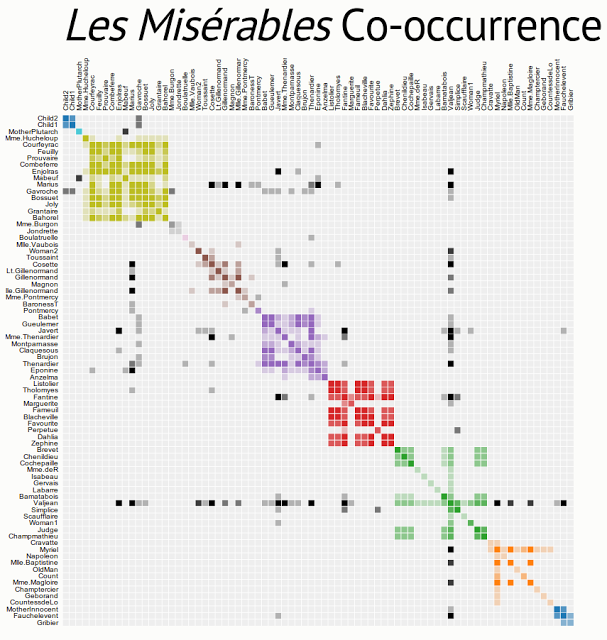
\includegraphics[width=\columnwidth]{mat-co}
 
 \caption{co-occurence matrix}
 \label{fig:mat-co}
\end{figure} 


\subsection{Juxtaposition}
As Jean-Daniel Fekete\cite{Fekete} wrote, one drawback of adjacency matrix is that some informations about the topological properties of graphs are lost, as instance, there is no way to represent where Marseille is located to Paris or Lyon or etc... The juxtaposition of a graph in order to represent the topological aspect of those data must be done if some geographical aspects are correlated. It is also important to notice that adjacency matrix does not provide a way to represent path between multiple nodes as instance the path between Paris, Lyon and Marseille, there will be visualize in a convenient way. As a consequence, if there is no direct path between two cities, there will be no way to represent it. Again, adding a graph or a map of the subject will provide some good support for the visualisation of the problem. 
Now the point is what can we juxtapose next to the adjacency matrix and what additional information this juxtaposed visualisation provides?
\begin{itemize}
\item Barcharts and linecharts: this representation can be a good way to decompose the data over time and then show some evolution of trends.
\item Trendalyzer, if we can correlate different populations of data in order to show a trend, we can use this well known representation.
\item Graph and maps: in order to introduce data in a geographical context graph and maps are required.
\end{itemize}
\subsection{NodeTrix}
As said before\cite{nodetrix}, the representation of dense graph is problematic so adjacency matrix is a good way to condense data, but we are losing some information. As we have seen before, the juxtaposition provides a solution to this problem. But the problem of the juxtaposition is that we have multiple representation and correlate in the same time. So instead of condensing all the data, the graph can be reduced by aggregating nodes of the same area, this will give a smaller graph. Now with this graph we can represent every nodes by a adjacency matrix and as a result, the visualisation still have a topological representation. This is in theory a good representation of data but in practice it can be hard to find a good way to cluster the data.

Moreover, the exhaustivity of the information is not well represented in the adjacency matrix so one idea is to juxtapose some additional graphics such as barchart in order to give statistics and evolutions about the links between cities.

\section{Design}
\subsection{Datasets}
We choose to work on the delayed train and how to visualize the fact that people thinks that trains are always late. For this project we are using an open dataset from the SNCF website. The dataset is composed of the train station, with traffic regularity rate and the date of the measures. Those data will provide some geographical informations that we must keep in the visualisation of the problem in order to give to the audience concrete results.



\subsection{Visualization}
The relevance of adjacency matrix for our problem is showed by the fact that we have too much data to represent in a single map, as we can see in (figure 1) we will represent the delayed train traffic by the color of the square corresponding to this travel, for example, between $90\%$ and $100\%$ regularity we will color the square in green, between $85\%$ and $90\%$ a yellow square and red and black squares for the lowest regularity and of course white square for no link between two train stations. Obviously the lack of geographical representation of the train station will be a crucial point to solve. One way to solve it is to use this concept of juxtaposition in order to give some additional data to visualize in a map for example. We can also use trix map in order to join together the train stations which are topologically close together such as Part Dieu, Perrache, Vaise. One issue which have been mentioned above is that we don’t know if the data have chosen will fit with this concept. (do we have enough train stations close together?) We can also cluster the graph with cardinal points and then make adjacency matrix for each of them. 
In terms of juxtaposed data we can use barcharts in order to visualize data versus time with a more precise granularity and in a more targeted area. As instance we can click on a square of the adjacency matrix (as instance Paris-Lyon) and then we will be able to visualize how traffic regularity is evolving in Lyon Paris line in a year or even more.
We can also add a little sample of the graph by clicking on several squares of the adjacency matrix and the representation will provide some topological contexts, it will also give to the audience some information about a path. As instance if we click on Paris -Lyon and Lyon - Marseille, the representation of the graph Paris, Lyon, Marseille will give to the audience some informations about this correspondence.



\begin{figure}[h!]
 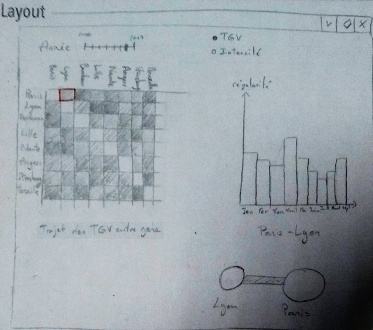
\includegraphics[width=\columnwidth]{first-layout}
 
 \caption{Design}
 \label{fig:sample}
\end{figure} 
\section{Conclusion}
To conclude, adjacency matrix is a solid way to visualize graph data and to condense information. But the main problem is that we are losing too much information(about topological aspects and multiple node paths \cite{Fekete} so using the juxtaposition is a good way to give to our problem a better context and some additional statistics and trends.

\bibliographystyle{plain}
\bibliography{mybib}

\end{document}